\documentclass{report}
\usepackage{setspace}
\usepackage{contour}
\usepackage{ulem}
\usepackage{caption}
\usepackage{subcaption}
\usepackage{geometry}
\usepackage{multicol}
\usepackage{array,etoolbox}
\usepackage{fancyhdr}
\usepackage{enumitem}
\usepackage[toc,page]{appendix}
\geometry{
letterpaper,
left=1in,
right=1in,
bottom=1in,
top=1in,
}

\pagestyle{fancy}
\lhead{PeaPod - Design Brief}
\rhead{UTAG}

\newcounter{metricnumber}
\setcounter{metricnumber}{1}
\newcommand\metricrow{M\arabic{metricnumber}}

% \renewcommand{\baselinestretch}{1.5}
\setstretch{1.5}

\begin{document}

\begin{titlepage}
    \begin{center}
        \vspace*{1.2cm}
        
        \textbf{\large{PeaPod - Design Brief}}
        
        \vspace{0.5cm}
        Outlining the Requirements for a Submission to the \\NASA/CSA Deep Space Food Challenge - Phase 1

        \vfill
        
        Jayden Lefebvre - Lead Engineer\\\small{jayden.lefebvre@mail.utoronto.ca}
        
        \vspace{2.5cm}
        
        Revision 0.4\\
        University of Toronto Agritech\\
        May 18th, 2021
        
    \end{center}
 \end{titlepage}

\thispagestyle{plain}

\tableofcontents
\newpage

\section{Introduction}
\label{sec:intro}

\subsection{Purpose}
\label{sec:purpose}

The purpose of this design brief is to outline the requirements for a submission 
to the NASA/CSA Deep Space Food Challenge Phase 1 \cite{dsfc}. In doing so, it also
documents the scope of a design submitted by University of Toronto Agritech (UTAG).

The goal of the Deep Space Food Challenge is for participants to "Create novel 
food production technologies or systems that require \uline{minimal inputs} and \uline{maximize safe}, nutritious, and palatable food outputs for 
\uline{long-duration space missions}, and which have potential to benefit 
people on Earth." \cite{applicantguide}

\subsection{Framing Structure}
\label{sec:structure}

This document achieves its purpose via "top-down" framing (Section \ref{sec:framing}), with each subsection's 
entries being derived from the entries of the previous\footnote{Each objective and metric has 
a numbered reference to the entry it was derived from (\uline{\textbf{S}}takeholder 
\uline{\textbf{1}} : S1, \uline{\textbf{H}}igh-\uline{\textbf{L}}evel Objective 
\uline{\textbf{8}} : HL8, etc.)}.

\begin{itemize}
    \item \textbf{\ref{sec:opportunity} - Opportunity}: A succinct scoped challenge 
    statement.
    \item \textbf{\ref{sec:requirements} - Challenge Requirements}: Categorical/unscoped 
    requirements for \textit{any} submission.
    \item \textbf{\ref{sec:stakeholders} - Stakeholders}: Persons and groups in 
    consideration.
    \item \textbf{\ref{sec:hlos} - High-Level Objectives}: Conceptual aims, DfX; derived 
    from Requirements and Stakeholders.
    \item \textbf{\ref{sec:llos} - Low-Level Objectives}: Tactical goals; derived from HLOs.
    \item \textbf{\ref{sec:metrics} - Metrics}: Quantitative measures of design success, fit, 
    utility, etc.; derived from LLOs.
    \item \textbf{\ref{sec:constraints} - Constraints}: Scoped \textit{mandatory} requirements for 
    the proposed design.
    \item \textbf{\ref{sec:criteria} - Criteria}: Scoped \textit{optional} requirements for 
    the proposed design.
\end{itemize}

In addition to framing the challenge, this document serves to outline the structural requirements 
of the Phase 1 prototypes (See Appendices \ref{sec:assessment}, \ref{sec:application}).

\newpage

\subsection{Scope and Justification}
\label{sec:scope}

Phase 1 development, testing, and assessment is scoped to terrestrial/Earth-like operational constraints \cite{applicantguide}:
\begin{itemize}
    \item Gravity (9.81 m/s${}^2$);
    \item Ambient atmospheric pressure (101,325 Pa);
    \item Ambient atmospheric/"room" temperature (22 °C);
    \item Ambient atmospheric humidity (50 \%RH);
\end{itemize}

In addition, it is important to note that the solution "need not meet the full nutritional requirements of 
future crews, but can contribute significantly to, and integrate with, a comprehensive food system." \cite{applicantguide} 
However, in implementation it can be assumed that this would be the only crop growth system on-board, and as such would
need to provide the majority.

The three underlined criteria in the challenge statement in Section \ref{sec:purpose} have also helped to define the 
scope of this brief:

\begin{enumerate}
\item The longer the duration of the space mission (up to and including interplanetary 
    travel and permanent colonization) the lesser the feasability of resupply
    \footnote{Minimal resupply is also listed as a constraint directly in the challenge 
    details \cite{applicantguide}.}.
\item The lesser the feasability of resupply, and the more minimal the input 
    (i.e. launch mass), the more the design will need to generate net-new food 
    grown on-board during the mission \footnote{Any other food production technologies 
    would be taking advantage of existing food; as such this is the basis for the 
    problem.}.
\item The minimization of inputs (launch mass), the minimization of other negative 
    criteria such as growth time, design complexity, etc. and the maximization of 
    safety (pathogenic and otherwise) means that food animal growth has been deemed 
    not feasible, and is outside the scope of this brief. Thus, the design should 
    focus on food-producing plant (or crop) growth\footnote{This is primarily an 
    issue in-transit; for colonization, non-plant food production systems should 
    definitely be considered.}.
\item Spacecraft are not good crop growth systems (lack of water access, proper 
    lighting and nutrition, etc.), thus the design should encompass a crop growth 
    environment that:
    \begin{enumerate}
        \item provides of all necessary crop growth inputs (water, nutrients, lighting, 
        etc.);
        \item contains or otherwise encompasses a viable crop growth environment 
        (temperature, humidity, gas concentrations, airflow, etc.);
        \item has control over all parameters of both a) and b) (environment parameters); 
        these together are the (crop growth) environment conditions.
    \end{enumerate}
\item To maximise safety (of both the crops and the crew) and redundancy, and to minimize 
    inputs (required human interaction), the environment should be automated and isolated 
    from the spacecraft cabin with regards to all environment conditions (thermally, 
    water-tight, etc.) unless beneficial and efficient (i.e no loss).
\item A greater degree of nutrition and palatability of food outputs implies a greater 
    variety of crops (incl. leafy greens, fruits/fruiting vegetables, root vegetables, 
    algaes, etc.); as such the food production system should be able to generate a 
    continuous variety of environmental conditions such that any number of food crops 
    could be grown within.
\item The demand for high crop variety, automation, parameter control, etc. implies 
    the use of a hydroponic/aeroponic/hybrid crop growth method.
\item Output nutrient and yield maximization in a controlled-environment implies environment
    parameter optimization. This is best accomplished via collection of both plant-growth and 
    environment metrics and cross-growth-environment networking 
    (data versatility, sharing, and machine intelligence).
\end{enumerate}

\newpage

\subsection{Definitions}
\label{sec:definitions}
A number of useful definitions have emerged from the above scoping:

\begin{enumerate}
\item \textbf{(Crop Growth) Environment} - The environment within which the crop grows/with which 
the crop interacts; the Environment Parameters in terms of their relationship with the 
crop and its growth.
\item \textbf{(Crop Growth) Environment Parameters} - The (often quantitative) parameters of the 
Crop Growth Environment, as well as any and all other parameters influencing crop growth.
\item \textbf{Crop Growth System} - Includes the physical enclosure (containing the crops and the 
controlled environment; incl. isolation) as well as any infrastructure required to 
generate the crop growth environment and control all environment conditions; satisfies 
all requirements of this brief.
\item \textbf{Crop Growth Metrics} - The (often quantitative) measures of crop growth optimization,
    including yield mass, growth rate, nutrient/etc. concentrations, etc.
\item \textbf{Environment Program} - The to-date most optimized set of Environment Parameters 
for a given Crop Growth Metric, implemented by the Grop Growth System.
\end{enumerate}

\section{Framing}
\label{sec:framing}

\subsection{Opportunity}
\label{sec:opportunity}

Design a fully automated and isolated hydroponic/aeroponic crop growth system for the 
Deep Space Food Challenge Phase 1\cite{dsfc}, able to generate any environment from a 
combination of independent environment parameters, with crop-growth and environment data
collection.

\newpage

\subsection{Challenge Requirements}
\label{sec:requirements}

The following are the overall challenge requirements compiled from DSFC Applicant Guide details \cite{applicantguide} and an excerpt of NASA-STD-3001: Section 7.1 Food and Nutrition\footnote{Additional nutrition and caloric output constraints relative to activity level, crew details, etc. are provided; however they are not in direct consideration as of Phase 1.} \cite{nutrition}:
\begin{enumerate}[label=R\arabic*., ref=R\arabic*]
    \item \label{r:1} \textbf{Must} help fill food gaps for a \textit{three-year} round-trip mission with 
    \textit{no resupply}:
    \begin{enumerate}[ref=R1\alph*]
        \item \label{r:1a} \textbf{Should} aim to produce food outputs that fulfill \textbf{all 
        daily nutritional needs} for a crew of \textit{four (4)} people;
        \item \label{r:1b} \textbf{Must} maintain food output \textit{safety} and \textit{nutrition} during \textit{all phases} of the mission;
        \item \label{r:1c} \textbf{Must} output food that is \textit{acceptable} to the crew for the \textit{duration} of the mission;
        \item \label{r:1d} \textbf{Must} produce \textit{varied palatable} food outputs that require \textit{no additional processing time}\footnote{It is 
        assumed that fresh (or packaged unprepared) edible plant products are already 
        prepared on existing space missions, and that this preparation meets this requirement.};
    \end{enumerate}
    \item \label{r:2} \textbf{Should} improve the accessibility of food on Earth; in particular, via production 
    directly in urban centres and in remote and harsh environments:
    \begin{enumerate}[ref=R2\alph*]
        \item \label{r:2a} \textbf{Should} enhance local production;
        \item \label{r:2b} \textbf{Should} reduce food supply chain shortages;
        \item \label{r:2c} \textbf{Should} reduce the impact on the resources needed for food production;
        \item \label{r:2d} \textbf{Should} be able to operate in harsh and remote environments;
    \end{enumerate}
    \item \label{r:3} \textbf{Must} aim to achieve the \textit{greatest of food output} with \textit{minimal inputs} and \textit{minimal waste};
    \item \label{r:4} \textbf{Must} transmit \textit{operational data and limited video} to a remote location, and be able to receive periodic \textit{operational commands}.
    \item \label{r:5} \textbf{Must} operate under Earth-like conditions (See Section \ref{sec:scope});
    % TODO: more?
\end{enumerate}

\setstretch{1}

\newpage

\subsection{Stakeholders}
\label{sec:stakeholders}

\begin{enumerate}[label=S\arabic*., ref=S\arabic*]
    \item \label{s:1} Food Product Consumers - Palatability, output
    \item \label{s:2} NASA/CSA Stakeholders - Feasability, input, optimization
\end{enumerate}

\subsection{Objectives}
\label{sec:objectives}

\begin{multicols}{2}[\subsubsection{High-Level}\label{sec:hlos}]
    \begin{enumerate}[label=HL\arabic*., ref=HL\arabic*]
        \item \label{hl:1} Food Output Suitability \hfill (\ref{s:1}, \ref{r:1}, \ref{r:1a}, \ref{r:2a})
        \item \label{hl:2} Environment Control, Automation, and Optimization \hfill (\ref{s:2}, \ref{r:1b}, \ref{r:2c}, \ref{r:2d}, \ref{r:3}, \ref{r:4})
        \item \label{hl:3} Efficiency \hfill (\ref{s:1}, \ref{s:2}, \ref{r:1}, \ref{r:2a}, \ref{r:2c}, \ref{r:3})
        \item \label{hl:4} Cross-Contamination \hfill (\ref{s:1}, \ref{s:2}, \ref{r:1c})
        % \item \label{hl:5} Safety, Redundancy \hfill (\ref{s:1}, \ref{s:2}, \ref{r:1b}, \ref{r:2b})
        % \item \label{hl:6} Modularity, Repairability \hfill (\ref{s:1}, \ref{s:2}, \ref{r:2d})
        \item \label{hl:7} Feasability \hfill (\ref{s:2}, \ref{r:2c})
    \end{enumerate}
\end{multicols}

\begin{multicols}{2}[\subsubsection{Low-Level}\label{sec:llos}]
    \begin{enumerate}[label=LL\arabic*., ref=LL\arabic*]
        \item \label{ll:1} Output Food Variety \hfill (\ref{hl:1})
        \item \label{ll:2} Output Food Palatability \hfill (\ref{hl:1})
        \item \label{ll:3} Nutrient Output \hfill (\ref{hl:1}, \ref{hl:3})
        \item \label{ll:4} Energy Output \hfill (\ref{hl:1}, \ref{hl:3})
        \item \label{ll:5} Air Temperature Control \hfill (\ref{hl:2})
        \item \label{ll:6} Air Humidity Control \hfill (\ref{hl:2})
        % \item \label{ll:7} Gas Concentration Control \hfill (\ref{hl:2})
        \item \label{ll:8} Lighting Control \hfill (\ref{hl:2})
        \item \label{ll:9} Light Isolation \hfill (\ref{hl:2}, \ref{hl:3})
        \item \label{ll:10} Thermal Isolation \hfill (\ref{hl:2}, \ref{hl:3})
        \item \label{ll:11} Water-tightness \hfill (\ref{hl:2}, \ref{hl:4})
        \item \label{ll:12} Airflow \hfill (\ref{hl:2}, \ref{hl:4})
        \item \label{ll:13} Water Flow Rate \hfill (\ref{hl:2})
        \item \label{ll:14} Water Temperature \hfill (\ref{hl:2})
        \item \label{ll:15} Germination Success \hfill (\ref{hl:2})
        \item \label{ll:16} High Degree of Automation \hfill (\ref{hl:3}, \ref{hl:4})
        \item \label{ll:17} Energy Efficiency \hfill (\ref{hl:3})
        \item \label{ll:18} Water Usage Efficiency \hfill (\ref{hl:3})
        % \item \label{ll:19} Plant Matter Usage \hfill (\ref{hl:3})
        % \item \label{ll:20} Gas Exchange Incentive \hfill (\ref{hl:3})
        % \item \label{ll:21} Number of Harvests \hfill (\ref{hl:3})
        \item \label{ll:22} Time-To-Harvest/-Reharvest \hfill (\ref{hl:3})
        \item \label{ll:23} Germination Time \hfill (\ref{hl:3})
        \item \label{ll:24} Growth Time \hfill (\ref{hl:3})
        \item \label{ll:25} Potential for Cross-Contamination \hfill (\ref{hl:4})
        % \item \label{ll:26} Structural Safety \hfill (\ref{hl:5})
        % \item \label{ll:27} Electrical/Power Safety \hfill (\ref{hl:5})
        % \item \label{ll:28} Power Supply Redundancy \hfill (\ref{hl:5})
        % \item \label{ll:29} Infrastructure Redundancy \hfill (\ref{hl:5})
        % \item \label{ll:30} Growth Container Modularity \hfill (\ref{hl:6})
        % \item \label{ll:31} Infrastructure Modularity Support \hfill (\ref{hl:6})
        % \item \label{ll:32} Growth Container Repairability \hfill (\ref{hl:6})
        % \item \label{ll:33} Infrastructure Repairability \hfill (\ref{hl:6})
        % \item \label{ll:34} Documentation Completion \hfill (\ref{hl:6})
        % \item \label{ll:35} Design Complexity \hfill (\ref{hl:6})
        % \item \label{ll:36} Tool Speciality and Number \hfill (\ref{hl:6})
        \item \label{ll:37} Cost \hfill (\ref{hl:7})
        \item \label{ll:38} Size \hfill (\ref{hl:7})
    \end{enumerate}
\end{multicols}

\newpage

\subsection{Metrics}
\label{sec:metrics}

\begin{tabular}{| @{\makebox[2.2em][l]{\metricrow}} | p{8.7cm} | p{5.9cm} |} 
    \hline
    \multicolumn{1}{| @{\makebox[2.2em][l]{\textbf{\#}}} | l |}{\textbf{Metric}} & \textbf{Units}\\ 
    \hline
    Variety of Suitable Crops \refstepcounter{metricnumber}\label{m:1} \hfill (\ref{ll:1}) & Y/N (per crop) \\
    \hline
    % TODO: ref hedonic scale
    Palatability of Crop Output vs. Commercial \refstepcounter{metricnumber}\label{m:2} \hfill (\ref{ll:2}) & 1-10 Hedonic (per crop) \\
    \hline
    Crop Nutrient Concentration vs. Commercial \refstepcounter{metricnumber}\label{m:3} \hfill (\ref{ll:3}) & \% (per crop) \\
    \hline
    % Protein Output Density \refstepcounter{metricnumber}\label{m:4} \hfill (\ref{ll:3}) & g/kg \\
    % \hline
    % Protein Output \refstepcounter{metricnumber}\label{m:5} \hfill (\ref{ll:3}) & kCal/crewmember (\%TDEI) \\
    % \hline
    % Carbohydrate Output \refstepcounter{metricnumber}\label{m:6} \hfill (\ref{ll:3}) & kCal/crewmember (\%TDEI) \\
    % \hline
    % Lipid Output \refstepcounter{metricnumber}\label{m:7} \hfill (\ref{ll:3}) & kCal/crewmember (\%TDEI) \\
    % \hline
    % $\Omega$-6 Fatty Acid Output \refstepcounter{metricnumber}\label{m:8} \hfill (\ref{ll:3}) & g/day/crewmember \\
    % \hline
    % $\Omega$-3 Fatty Acid Output \refstepcounter{metricnumber}\label{m:9} \hfill (\ref{ll:3}) & g/day/crewmember \\
    % \hline
    % Saturated Fat Output \refstepcounter{metricnumber}\label{m:10} \hfill (\ref{ll:3}) & kCal/crewmember (\%TDEI) \\
    % \hline
    % Trans Fatty Acids Output \refstepcounter{metricnumber}\label{m:11} \hfill (\ref{ll:3}) & kCal/crewmember (\%TDEI) \\
    % \hline
    % Cholesterol Output \refstepcounter{metricnumber}\label{m:12} \hfill (\ref{ll:3}) & mg/day/crewmember \\
    % \hline
    % Fiber Output \refstepcounter{metricnumber}\label{m:13} \hfill (\ref{ll:3}) & g/day/crewmember \\
    % \hline
    Crew Nutrient Requirement Coverage \refstepcounter{metricnumber}\label{m:14} \hfill (\ref{ll:3}) & \% (best crop combo) \\
    \hline
    Caloric Output per Day \refstepcounter{metricnumber}\label{m:15} \hfill (\ref{ll:4}) & kCal/24hr (best crop combo) \\
    \hline
    Air Temperature Control Range \refstepcounter{metricnumber}\label{m:16} \hfill (\ref{ll:5}) & min, max °C \\
    \hline
    Air Temperature Control Rate \refstepcounter{metricnumber}\label{m:17} \hfill (\ref{ll:5}) & $\Delta$°C/sec at each °C \\
    \hline
    Air Temperature Control Stability \refstepcounter{metricnumber}\label{m:18} \hfill (\ref{ll:5}) & $\pm$°C at each °C \\
    \hline
    Air Humidity Control Range \refstepcounter{metricnumber}\label{m:19} \hfill (\ref{ll:6}) & min, max \%RH \\
    \hline
    Air Humidity Control Rate \refstepcounter{metricnumber}\label{m:20} \hfill (\ref{ll:6}) & $\Delta$\%RH/sec at each \%RH \\
    \hline
    Air Humidity Control Stability \refstepcounter{metricnumber}\label{m:21} \hfill (\ref{ll:6}) & $\pm$\%RH at each \%RH \\
    \hline
    % CO${}_2$ Concentration Control Range \refstepcounter{metricnumber}\label{m:22} \hfill (\ref{ll:7}) & min, max ppm CO${}_2$ \\
    % \hline
    % CO${}_2$ Concentration Control Rate \refstepcounter{metricnumber}\label{m:23} \hfill (\ref{ll:7}) & ppm CO${}_2$/sec at each ppm 
    % CO${}_2$ \\
    % \hline
    % CO${}_2$ Concentration Control Stability \refstepcounter{metricnumber}\label{m:24} \hfill (\ref{ll:7}) & $\pm$ppm CO${}_2$ at 
    % each ppm CO${}_2$ \\
    % \hline
    % O${}_2$ Concentration Control Range \refstepcounter{metricnumber}\label{m:25} \hfill (\ref{ll:7}) & min, max ppm O${}_2$ \\
    % \hline
    % O${}_2$ Concentration Control Rate \refstepcounter{metricnumber}\label{m:26} \hfill (\ref{ll:7}) & ppm O${}_2$/sec at each ppm 
    % O${}_2$  \\
    % \hline
    % O${}_2$ Concentration Control Stability \refstepcounter{metricnumber}\label{m:27} \hfill (\ref{ll:7}) & $\pm$ppm O${}_2$ at each 
    % ppm O${}_2$ \\
    % \hline
    Light Spectrum Wavelength Range \refstepcounter{metricnumber}\label{m:28} \hfill (\ref{ll:8}) & min, max nm \\
    \hline
    Light Spectrum PAR Match \refstepcounter{metricnumber}\label{m:29} \hfill (\ref{ll:8}) & \% (each crop) \\
    \hline
    Light Intensity Control Range \refstepcounter{metricnumber}\label{m:30} \hfill (\ref{ll:8}) & min, max $\mu$mol 
    m${}^{-2}$sec${}^{-1}$ at each nm \\
    \hline
    Light Intensity Control Stability \refstepcounter{metricnumber}\label{m:31} \hfill (\ref{ll:8}) & $\pm\mu$mol 
    m${}^{-2}$sec${}^{-1}$ at each nm \\
    \hline
    Light Loss, Capture by Surfaces \refstepcounter{metricnumber}\label{m:32} \hfill (\ref{ll:9}) & \% \\
    \hline
    Outside Light Penetration \refstepcounter{metricnumber}\label{m:33} \hfill (\ref{ll:9}) & \% \\
    \hline
    Heat Loss \refstepcounter{metricnumber}\label{m:34} \hfill (\ref{ll:10}) & $\pm$W at each °C \\
    \hline
    Water Loss due to Leaks, Evaporation \refstepcounter{metricnumber}\label{m:35} \hfill (\ref{ll:11}) & mL/hr \\
    \hline
    Internal Circulation Airflow Control Range \refstepcounter{metricnumber}\label{m:36} \hfill (\ref{ll:12}) & min, max m${}^3$/min \\
    \hline
    Gas Exchange due to Leaks \refstepcounter{metricnumber}\label{m:37} \hfill (\ref{ll:12}) & m${}^3$/min \\
    \hline
    Maximum Intentional Gas Exchange \refstepcounter{metricnumber}\label{m:38} \hfill (\ref{ll:12}) & m${}^3$/min \\
    \hline
    Nutrient Solution Delivery Control Range \refstepcounter{metricnumber}\label{m:39} \hfill (\ref{ll:13}) & min, max 
    mL/sec \\
    \hline
    Nutrient Solution Delivery Control Rate \refstepcounter{metricnumber}\label{m:40} \hfill (\ref{ll:13}) & $\Delta$mL/sec${}^2$ at each mL/sec  \\
    \hline
    Nutrient Solution Delivery Control Stability \refstepcounter{metricnumber}\label{m:41} \hfill (\ref{ll:13}) & 
    $\pm$mL/sec at each mL/sec \\
    \hline
% \end{tabular}
% \newpage

% \textbf{\large{2.5 \ \ Metrics (Cont'd)}}
% \normalsize

% \begin{tabular}{| @{\makebox[2em][l]{\metricrow}} | p{11.5cm} | p{3.2cm} |} 
    % \hline
    % \multicolumn{1}{| @{\makebox[2em][l]{\textbf{\#}}} | l |}{\textbf{Metric}} & \textbf{Units}\\ 
    % \hline
    Nutrient Solution Temp. Control Range \refstepcounter{metricnumber}\label{m:42} \hfill (\ref{ll:14}) & min, max °C \\
    \hline
    Nutrient Solution Temp. Control Rate \refstepcounter{metricnumber}\label{m:43} \hfill (\ref{ll:14}) & °C/sec at each °C  \\
    \hline
    Nutrient Solution Temp. Control Stability \refstepcounter{metricnumber}\label{m:44} \hfill (\ref{ll:14}) & 
    $\pm$°C at each °C  \\
    \hline
    Germination Success Rate \refstepcounter{metricnumber}\label{m:45} \hfill (\ref{ll:15}) & \% \\
    \hline
    Time Requirement - Maintenance \refstepcounter{metricnumber}\label{m:46} \hfill (\ref{ll:16}) & hrs/week \\
    \hline
    Time Requirement - Setup \refstepcounter{metricnumber}\label{m:47} \hfill (\ref{ll:16}) & hrs \\
    \hline
    Energy Efficiency - Power vs. kCal \refstepcounter{metricnumber}\label{m:48} \hfill (\ref{ll:17}) & \% \\
    \hline
    Necessary Water Waste per Day \refstepcounter{metricnumber}\label{m:49} \hfill (\ref{ll:18}) & L/day \\
    \hline
    % Water Recycling from Spacecraft Systems \refstepcounter{metricnumber}\label{m:50} \hfill (\ref{ll:18}) & L/day \\
    % \hline
    Initial Water Requirement \refstepcounter{metricnumber}\label{m:51} \hfill (\ref{ll:18}) & L \\
    \hline
    % Plant Matter Usage \refstepcounter{metricnumber}\label{m:52} \hfill (\ref{ll:19}) & \% \\
    % \hline
    % CO${}_2$ Capture - Fraction of Typical Reclaimer Consumption \refstepcounter{metricnumber}\label{m:53} \hfill (\ref{ll:20}) & \% \\
    % \hline
    % O${}_2$ Production - Fraction of Typical Reclaimer Production \refstepcounter{metricnumber}\label{m:54} \hfill (\ref{ll:20}) & \% \\
    % \hline
    % Number of Harvests per Planting \refstepcounter{metricnumber}\label{m:55} \hfill (\ref{ll:21}) & \# (each crop)\\
    % \hline
    Harvest to Reharvest - Fruiting Crops \refstepcounter{metricnumber}\label{m:56} \hfill (\ref{ll:22}) & min (each crop)  \\
    \hline
    Germination Time \refstepcounter{metricnumber}\label{m:57} \hfill (\ref{ll:23}) & min (each crop) \\
    \hline
    Seedling to Harvest \refstepcounter{metricnumber}\label{m:58} \hfill (\ref{ll:24}) & min (each crop) \\
    \hline
    Potential for Contamination - Germination \refstepcounter{metricnumber}\label{m:59} \hfill (\ref{ll:25}) & \% (each event)\\
    \hline
    Potential for Contamination - Planting \refstepcounter{metricnumber}\label{m:60} \hfill (\ref{ll:25}) & \% (each event)\\
    \hline
\end{tabular}
\newpage

\textbf{\large{2.5 \ \ Metrics (Cont'd)}}
\normalsize

\begin{tabular}{| @{\makebox[2.2em][l]{\metricrow}} | p{9.65cm} | p{4.9cm} |} 
    \hline
    \multicolumn{1}{| @{\makebox[2.2em][l]{\textbf{\#}}} | l |}{\textbf{Metric}} & \textbf{Units}\\ 
    \hline
    Potential for Contamination - Harvest \refstepcounter{metricnumber}\label{m:61} \hfill (\ref{ll:25}) & \% (each event)\\
    \hline
    % Factor of Safety \refstepcounter{metricnumber}\label{m:62} \hfill (\ref{ll:26}) & FOS (each structure)\\
    % \hline
    % Mounting Stability - System to Surroundings \refstepcounter{metricnumber}\label{m:63} \hfill (\ref{ll:26}) & FOS (each mount) \\
    % \hline
    % Mounting Stability - Infrastructure to System \refstepcounter{metricnumber}\label{m:64} \hfill (\ref{ll:26}) & FOS (each mount) \\
    % \hline
    % Risk of Electrical Malfunction \refstepcounter{metricnumber}\label{m:65} \hfill (\ref{ll:27}) & \% \\
    % \hline
    % Backup Power Systems? \refstepcounter{metricnumber}\label{m:66} \hfill (\ref{ll:28}) & Y/N \\
    % \hline
    % Incremental Power-On? \refstepcounter{metricnumber}\label{m:67} \hfill (\ref{ll:28}) & Y/N \\
    % \hline
    % Backup Water Systems? \refstepcounter{metricnumber}\label{m:68} \hfill (\ref{ll:29}) & Y/N \\
    % \hline
    % Infrastructure Failure Notification? \refstepcounter{metricnumber}\label{m:69} \hfill (\ref{ll:29}) & Y/N \\
    % \hline
    % Independent Crop Growth Environments? \refstepcounter{metricnumber}\label{m:70} \hfill (\ref{ll:30}) & Y/N \\
    % \hline
    % Support for N+1 Crop Growth Environments? \refstepcounter{metricnumber}\label{m:71} \hfill (\ref{ll:31}) & Y/N \\
    % \hline
    % Lighting System Swappable? \refstepcounter{metricnumber}\label{m:72} \hfill (\ref{ll:32}) & Y/N \\
    % \hline
    % Heating/Cooling System(s) Swappable? \refstepcounter{metricnumber}\label{m:73} \hfill (\ref{ll:32}) & Y/N \\
    % \hline
    % Water Delivery System(s) Swappable? \refstepcounter{metricnumber}\label{m:74} \hfill (\ref{ll:32}) & Y/N \\
    % \hline
    % Lighting System Swappable? \refstepcounter{metricnumber}\label{m:75} \hfill (\ref{ll:32}) & Y/N \\
    % \hline
    % Computer Subsystems Swappable? \refstepcounter{metricnumber}\label{m:76} \hfill (\ref{ll:33}) & Y/N \\
    % \hline
    % All Fabrication Procedures, Tools, and Materials Documented? \refstepcounter{metricnumber}\label{m:77} \hfill (\ref{ll:34}) & Y/N \\
    % \hline
    % All Assembly Procedures, Tools, and Materials Documented? \refstepcounter{metricnumber}\label{m:78} \hfill (\ref{ll:34}) & Y/N \\
    % \hline
    % All Repair Procedures, Tools, and Materials Documented? \refstepcounter{metricnumber}\label{m:79} \hfill (\ref{ll:34}) & Y/N \\
    % \hline
    % Total Fabrication, Assembly, and Startup Time \refstepcounter{metricnumber}\label{m:80} \hfill (\ref{ll:35}) & min \\
    % \hline
    % Total Number of Tools Required \refstepcounter{metricnumber}\label{m:81} \hfill (\ref{ll:36}) & \# \\
    % \hline
% \end{tabular}

% \newpage

% \textbf{\large{2.5 \ \ Metrics (Cont'd)}}
% \normalsize

% \begin{tabular}{| @{\makebox[2em][l]{\metricrow}} | p{11.5cm} | p{3.2cm} |} 
%     \hline
%     \multicolumn{1}{| @{\makebox[2em][l]{\textbf{\#}}} | l |}{\textbf{Metric}} & \textbf{Units}\\ 
%     \hline
    % Number of New Tools Required \refstepcounter{metricnumber}\label{m:82} \hfill (\ref{ll:36}) & \# \\
    % \hline
    Cost \refstepcounter{metricnumber}\label{m:83} \hfill (\ref{ll:37}) & CAD \\
    \hline
    Outer Dimensions \refstepcounter{metricnumber}\label{m:84} \hfill (\ref{ll:38}) & m (W, D, H) \\
    \hline
    Outer Volume \refstepcounter{metricnumber}\label{m:85} \hfill (\ref{ll:38}) & m${}^3$ \\
    \hline
    Power Consumption \refstepcounter{metricnumber}\label{m:86} \hfill (\ref{ll:38}) & W \\
    \hline
    Mass \refstepcounter{metricnumber}\label{m:87} \hfill (\ref{ll:38}) & kg \\
    \hline
\end{tabular}

\subsection{Constraints}
\label{sec:constraints}
\begin{tabular}{|l|p{12.55cm}|p{1.3cm}|}
    \hline
    \textbf{Metric} & \textbf{Constraint} & \textbf{Source} \\
    \hline
    M\ref{m:45} & 4 hrs/week & \cite{applicantguide}\\
    \hline
    M\ref{m:83} & Fits through 1.07m x 1.90m doorway; W<1.829m, D<2.438m, H<2.591m & \cite{applicantguide} \\
    \hline
    M\ref{m:84} & $\le$ 2 m${}^3$ & \cite{applicantguide}\\
    \hline
    M\ref{m:85} & Avg. <1500W; Peak < 3000W & \cite{applicantguide}\\
    \hline
\end{tabular}

\subsection{Criteria}
\label{sec:criteria}
\begin{tabular}{|l|p{12.55cm}|p{1.3cm}|}
    \hline
    \textbf{Metric} & \textbf{Criteria; Reason} & \textbf{Source} \\
    \hline
    M\ref{m:34} & Minimize; Reduce System Inputs & \cite{applicantguide} \\
    \hline
    M\ref{m:48} & Minimize; Reduce System Inputs & \cite{applicantguide} \\
    \hline
    M\ref{m:49} & Maximize; Reduce System Inputs & \cite{applicantguide} \\
    \hline
    % M\ref{m:50} & Minimize; Reduce System Inputs & \cite{applicantguide} \\
    % \hline
    M\ref{m:86} & Minimize; Reduce System Inputs & \cite{applicantguide} \\
    \hline
\end{tabular}

Refer to Appendix \ref{sec:assessment} for prototype verification Assessment Criteria (categories, weights, etc.).

\newpage

\begin{appendices}
\section{Assessment Criteria}
\label{sec:assessment}
\subsection{Report Assessment Criteria}
\label{sec:reportassessment}

\begin{figure}[h]
    \centering
    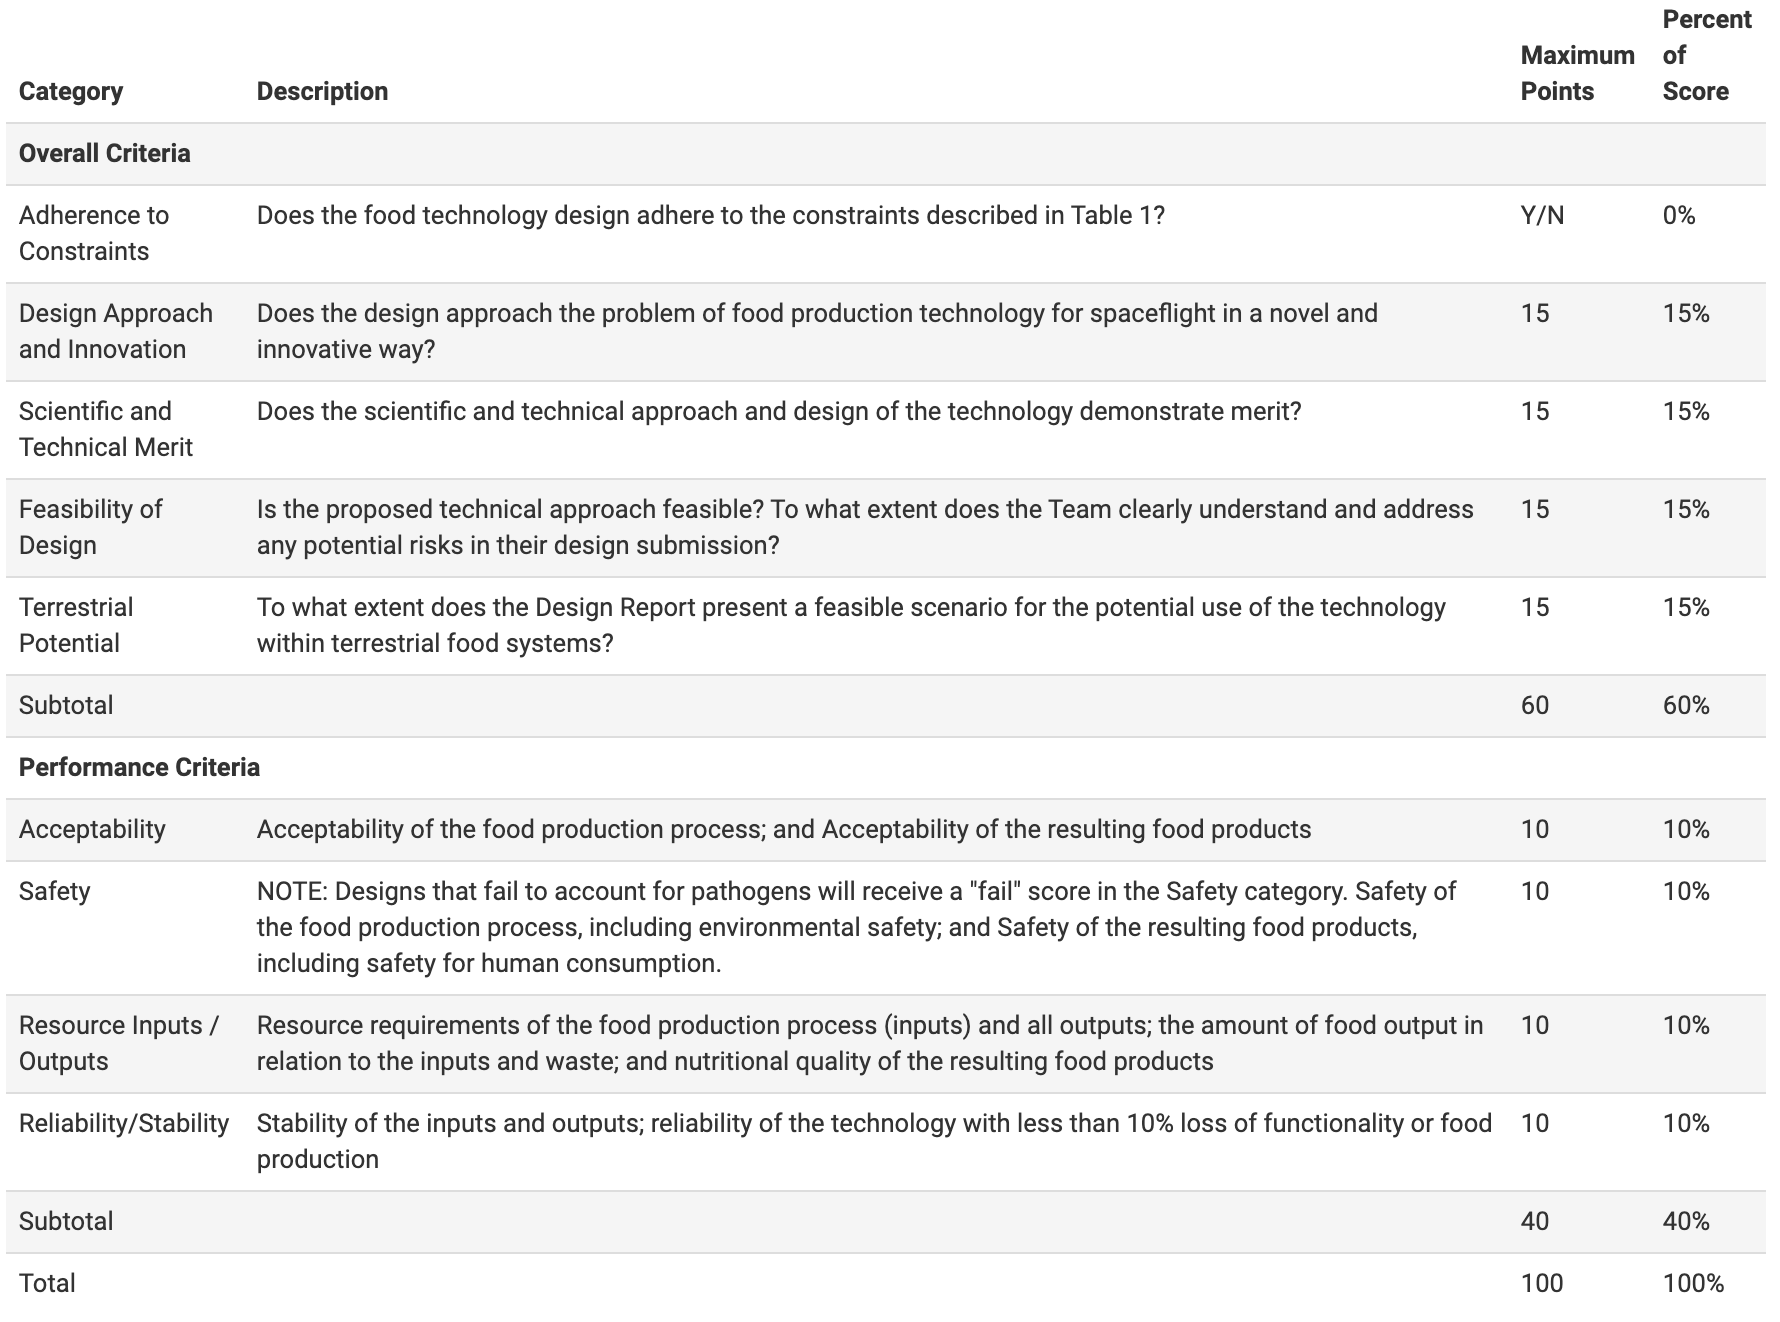
\includegraphics[width=15cm]{images/reportassessment.png}
    \hfill
    \caption{Design report assessment categories and weights \cite{applicantguide}.}
\end{figure}

\subsection{Animation Assessment Criteria}
\label{sec:animassessment}

\begin{figure}[h]
    \centering
    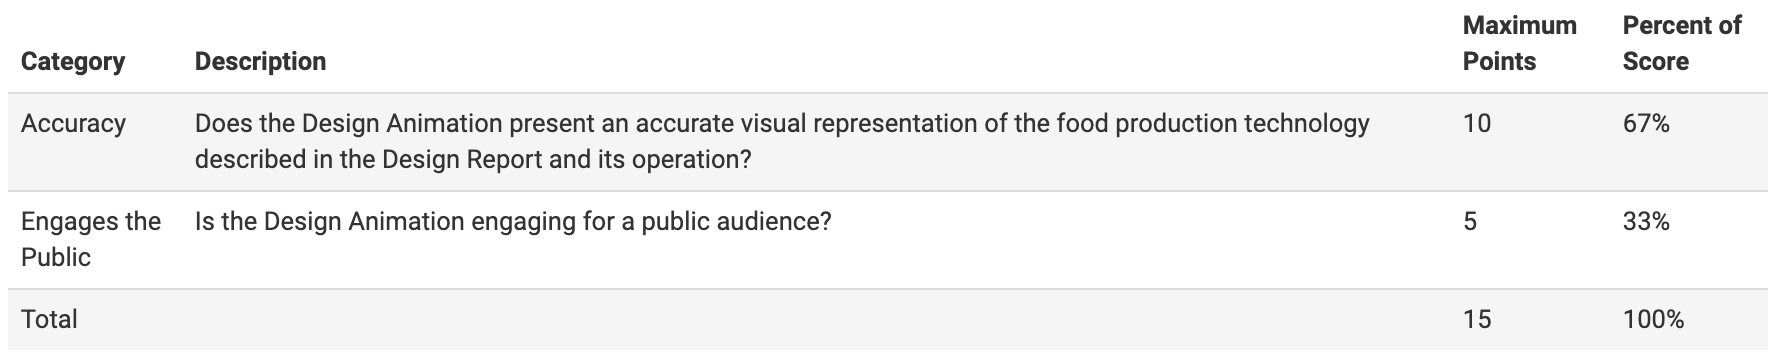
\includegraphics[width=15cm]{images/animassessment.png}
    \hfill
    \caption{Design animation assessment categories and weights \cite{applicantguide}.}
\end{figure}

\newpage

\section{Application Details}
\label{sec:application}

The contents of this appendix are adapted from \cite{applicantguide}, and should serve as the framework 
for developing the Phase 1 prototype.

A complete application package consists of the Challenge Application Form, with the following sections:

\begin{enumerate}
    \item Applicant details (basic information, primary contact);
    \item Proposed solution details:
    \begin{enumerate}
        \item Design Abstract;
        \item Design Report (See Appendix \ref{sec:reportassessment});
        \item Design Animation (video; See Appendix \ref{sec:animassessment});
        \item Intellectual Property Details;
    \end{enumerate}
    \item Declaration (terms and conditions, Consent for Use, Disclosure and Copyright requirements);
    \item Survey (optional);
\end{enumerate}

\end{appendices}

\newpage

\bibliographystyle{IEEEtran}

\bibliography{references}

\end{document}